\chapter{Introduction}
- INTRODUZIONE DELLA TESI E DEL LAVORO DI DOTTORATO (VEDI FIL)
- INTRODUZIONE SOMMARIA DEI PROBLEMI AFFRONTATI (CHE VERRA' POI APPROFONDITA IN CIASCUNA SECTION)

%% FILTRARE LA SEGUENTE INTRODUZIONE (CSUR18) 
Nowadays, the amount of public available information encourages the study and development of Sentiment Analysis algorithms that analyse huge amount of users' data with the aim to infer reactions about topics, opinions, trends to understand the mood of the users whose produce and share information through the web. The aim of Sentiment Analysis is to extract the attitude of people toward a topic or the intended emotional affect the author wishes to have on the readers. The tasks of this research field are challenging as well as very useful in practice. Sentiment analysis finds several practical applications, since opinions influence many human decisions either in business and social activities.  
%Sentiment analysis systems are being applied in almost every business and social domain because opinions are central to almost all human activities and are key influencers of our behaviours. 
As instance, companies are interested in monitoring people opinions toward their products or services, as well as customers rely on feedbacks of other users to evaluate a product before they purchase it.
%For example, companies always want to find public or consumer opinions toward their products and services. Furthermore, customers also want to know the opinions of other users before they use a service or purchase a product.
With the growth of social media (i.e., reviews, forums, blogs and social networks), individuals and organizations are increasingly using public opinions  for their decision making~\cite{liu2012survey}.
%The analysis of such social information enables applications such as brand monitoring, market prediction or political voting forecasting.
\\
ALLARGARE LE CATEGORIE DI TASK, INSERENDO LE DIVERSE ACCEZIONI DI SENTIMENT 
\\
SENTIMENT  ---> CONTENT POLARITY AND CONTENT POPULARITY
\\POLARITY   ---> POSITIVE / NEGATIVE EVOKED EMOTION ---> SENTIMENT PREDICTION
\\POPULARITY ---> POPULARITY ON SOCIAL PLATFORMS --> FLICKR
\\POPULARITY ---> POPULARITY IN SOCIAL EVENTS --> RECFUSION + TSP


The basic task in Sentiment Analysis is the polarity classification of an input text (e.g., taken from a review, a comment or a social post) in terms of positive, negative or neutral polarity. This analysis can be performed at document, sentence or feature level. The methods of this area are useful to capture public opinion about products, services, marketing, political preferences and social events. For example the analysis of the activity of Twitter's users can help to predict the popularity of parties or coalitions. The achieved results in Sentiment Analysis within micro-blogging have shown that Twitter posts reasonably reflect the political landscape~\cite{tumasjan2010predicting}.
Historically, Sentiment Analysis techniques have been developed for the analysis of text~\cite{pang2008opinion}, whereas limited efforts have been employed to extract (i.e., infer) sentiments from visual contents~(e.g., images and videos). % which are becoming a pervasive media on the web.
%Historically, the computational analysis of sentiment mostly concentrates on the textual contents~\cite{pang2008opinion}, whereas limited efforts have been conducted to analyse sentiments from visual contents such as images and videos, which are becoming a pervasive media type on the web.

Even though the scientific research has already achieved notable results in the field of textual Sentiment Analysis in different contexts (e.g., social network posts analysis, product reviews, political preferences, etc.), the task to understand the mood from a text has several difficulties given by the inherent ambiguity of the various languages (e.g., ironic sentences), cultural factors, linguistic nuances and the difficulty of generalize any text analysis solution to different language vocabularies. The different solutions in the field of text Sentiment Analysis have not yet achieved a level of reliability good enough to be implemented without enclosing the related context. For example, despite the existence of natural language processing tools for the English language, the same tools cannot be used directly to analyse text written in other languages.
Although NLP (Natural Language Processing) and information retrieval researchers proposed several approaches to address the problem of Sentiment Analysis~\cite{pang2008opinion}, the social media context offers some additional challenges. Beside the huge amounts of available data, typically the textual communications on social networks consist of short and colloquial messages. Moreover, people tend to use also images and videos, in addition to the textual messages, to express their experiences through the most common social platforms.
The information contained in such visual contents are not only related to semantic contents such as objects or actions about the acquired picture, but also cues about affect and sentiment conveyed by the depicted scene. Such information is hence useful to understand the emotional impact (i.e., the evoked sentiment) beyond the semantic.
For these reasons images and videos have become one of the most popular media by which people express their emotions and share their experiences in the social networks, which have assumed a crucial role in collecting data about people's opinions and feelings. %Nowadays, the diffusion of social networks plays a crucial role in collecting information about people opinion.
The images shared in social media platforms reflect visual aspects of users' daily activities and interests. Such growing user generated images represent a recent and powerful source of information useful to analyse users' interests. 
%The social images uploaded by users can be considered to reflect visual aspects of their daily activities and interests. Such growing user generated images represent a new source of information useful to analyse users' opinions. 
%The Sentiment Analysis of such large scale visual contents can help to better extract user moods regarding events or topics, so that Visual Sentiment Analysis is complementary to textual Sentiment Analysis.  
Extracting the emotions inherently underlying images perceived by the viewers could promote new approaches to several application fields such as brand perception, assessment of customer satisfaction, advertising, and media analytic, etc.
The diffusion of personal mobile devices constantly connected to Internet services (e.g., smartphones) and the growth of social media platforms introduced a new communication paradigm by which people that share multimedia data. %, by allowing new interaction models. 
In this context, uploading images to a social media platform is the new way by which people share their opinions and experiences.  
This provides a strong motivation for research on this field, and offers many challenging research problems.

This paper aims to introduce this emerging research field, analyse the related problems, provide a brief overview of current research progress, discuss the major issues and outline the new opportunities and challenges in this area.


The paper is organized as follows. In Section~\ref{stateoftheart} an overview of the most significant works in the field of Visual Sentiment Analysis, published between 2010 and 2018 is presented. The literature is presented in a chronological order, highlighting similarities and differences between the different works, with the aim to drive the reader along the evolution of the developed methods.
Section~\ref{systems} provides a complete overview of the system design choices, with the aim to provide a deepth debate about each specific issue related to the design of a Visual Sentiment Analysis systems: emotions representation schemes, existing datasets, features. Each aspect is discussed, and the different possibilities are compared one each other, with related references to the state of the art.
Section~\ref{problem} provides a complete formalization of the problem, by abstracting all the components that could affect the sentiment associated to an image, including the sentiment holder and the time factor, often ignored by the existing methods. References to the state of the art addressing each component are reported, as well as the different alternative solutions are proposed.
Section~\ref{challenges} introduces some additional challenges and techniques that could be investigated, proposing suggestions for new methods, features and datasets.
Then, Section~\ref{conclusions} reports the summary of the insights as outcome of the proposed study.

\section{Dissertation Structure}
- INTRODUZIONE DEI PAPER IN RELAZIONE AI TEMI DESCRITTI SOPRA
- DESCRIZIONE SOMMARIA DEI CAPITOLI SEGUENTI
\begin{figure}[t]
	\centering
	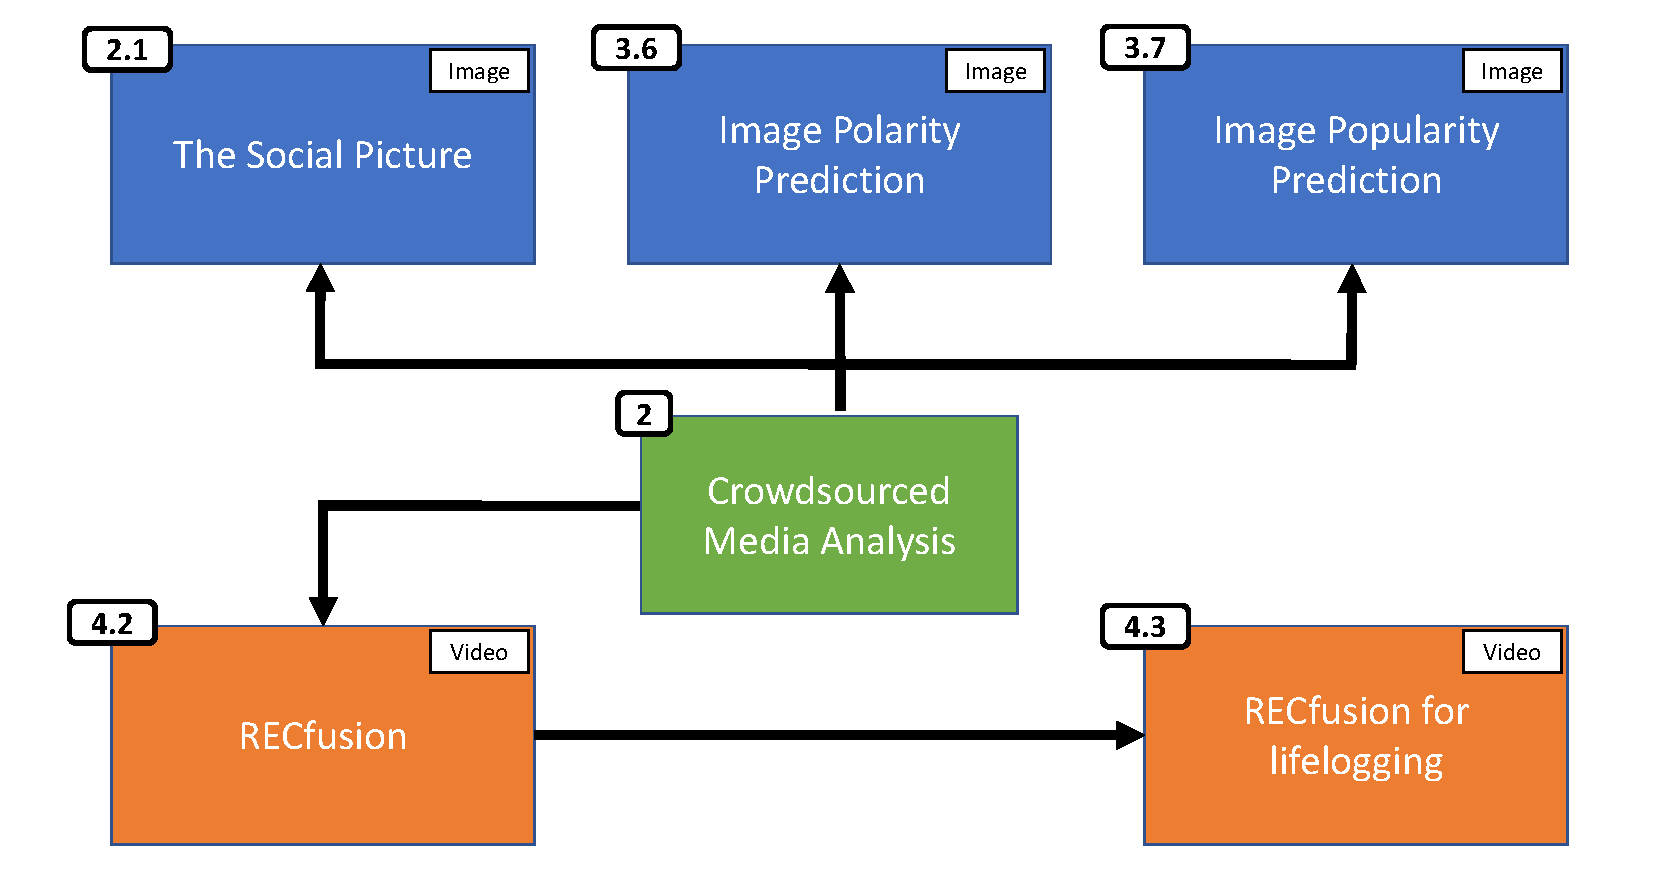
\includegraphics[width=1\linewidth]{schema.pdf}
	\caption{Dissertation structure
	}
	\label{figDissertationSchema}
\end{figure}


\section{List of Publications}